\chapter{Identification}
\section{Sputnik VAD}\label{Sputnik}
% graphic of Sputnik construction
The Sputnik VAD is an axial-flow blood pump, developed in a cooperative project of the National Research University of Electronic Technology, OJSC Zelenograd Innovation-Technology Center of Medical Equipment, FSBI "Academician V.I. Shumakov Federal Research Center of Transplantology and Artificial Organs", Ministry of Health of Russian Federation, DONA-M LLC and BIOSOFT-M LLC in 2009. \cite{Sputnik1}
\\This device is used for left ventricular assistance in patients with acute heart failure. The therapeutic objective in implantation of a Sputnik VAD is bridging to transplantation. The VAD is able to pump up to 10 liters of blood per minute with a continuous flow profile. The implantable pump weighs about $200\, g$, has a length of $81\, mm$ and a maximum diameter of $34\, mm$. It consists of a moving and a stationary part. The moving part, the impeller, a rotor with four blades, contains a permanent NdFeB-magnet, which is actuated by a brushless DC motor. The rotor spins clockwise with speed values between $4000-10000\, rpm$. An overview of the pump's specification is presented in \tablename~ \ref{tab:sput1}.
\begin{table}[ht]
  \centering
  \begin{tabular}{c|c}
    \toprule
    Blood flow  & 0-10 l/min \\
    Rotational speed & 4000-10000 rpm \\
    Length & 81 mm \\
    Diameter & 34 mm \\
    Weight & 200 g \\
    \bottomrule
\end{tabular}
  \caption[Specifications of Sputnik VAD]{Specifications of Sputnik VAD}
  \label{tab:sput1}
\end{table}
The stator is located inside a titanium housing with a $16\, mm$ diameter. The stationary part of the pump consists of a flow straightener with three stationary blades and a flow diffusor with three twisted blades. The flow straightener is located in front of the rotor and straightens the incoming blood flow into the rotor. Behind the rotor, blood is directed into the diffusor. %\cite{Sputnik1}
\figurename~ \ref{fig:sput_cross} depicts a cross-section of the Sputnik VAD and identifies its individual components.
The connection between the pump and the cardiovascular system is performed using in- and outflow cannulas, a felt ferule and vascular prosthesis which is sewed to the aorta. \cite{Sputnik1}
\begin{figure}[ht]
  \centering
  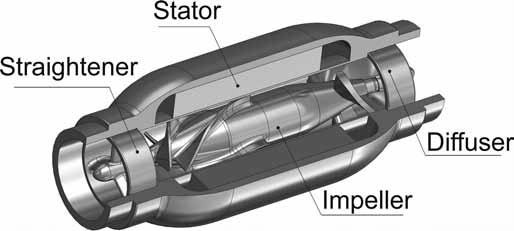
\includegraphics[width=0.6\textwidth]{images/chapt_4/sputnik_cross.png}
  \caption[Cross-section of Sputnik VAD \cite{Sputnik6}]{Cross-section of the Sputnik VAD \cite{Sputnik6}.}
  \label{fig:sput_cross}
\end{figure}
The Sputnik VAD is powered using two lithium-ion batteries, fully loaded providing enough energy for up to eight hours of system support. The maximum charging time for the batteries is less than five hours. During this time the batteries can either be exchanged by another set of batteries or the system can be powered through connection to an AC network. A microprocessor-based driving unit is used to regulate the pump speed, manage the power supply and store parameter data. It is connected percutaneously to the pump with an up to $170\, cm$ long and $5\, cm$ wide lead. \cite{Sputnik1}
\\During the practical part of this work the pump was controlled using the servo controller module ESCON 50/4 EC-S from maxon motor. This is a 4-quadrant pulse width modulation controller for controlling motors without Hall sensors.
%%%% ANSTEUERUNG ÜBER ESCON ERKLÄREN!!!

\section{Hardware in the Loop Test Bench}
For all measurements and tests performed during this thesis, a hardware in the loop (HiL) test bench of the Chair of Medical Information Technology at RWTH Aachen University was used. The test bench is implemented as a feedback controlled human circulatory system simulator. With the aid of the test rig, it is possible to test MCS systems under various physiological and pathological load patterns of the heart.
\begin{figure}[ht]
  \centering
  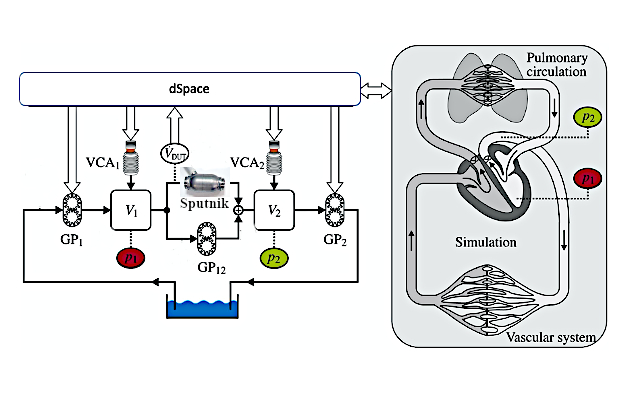
\includegraphics[width=\textwidth]{images/chapt_4/mock_loop.jpg}
  \caption[HiL test bench]{Structure of the HiL human ciculatory system simulator based on \cite{MCL}.}
  \label{fig:mock_loop}
\end{figure}
\\The structure of the mock circulatory loop (MCL) is depicted in \figurename~\ref{fig:mock_loop}. The boxes marked $V_{1}$ and $V_{2}$ are pressure compartments simulating the volume of the left ventricle and the aorta, respectively. Therefore, the pressure values of these compartments, referred to as $p_{1}$ and $p_{2}$, can be physiologically compared to the pressure values of the left ventricle and aorta. The MCL is actuated by three gear pumps ($GP_{1}$, $GP_{12}$ and $GP_{2}$) and two voice coil actuators ($VCA_{1}$ and $VCA_{2}$). The Sputnik VAD is connected to the pressure chambers in parallel, enabling tests similar to real use case. This way, the VAD can be subjected to comparable pressure changes in the differential pressure between the aorta and ventricle as would be the case when used on the beating heart.
\\By controlling the MCL through a dSpace system (DS1103), pressure in the chambers can be adjusted in real time to simulate different cardiac dysfunctions. The dSpace system furthermore enables recording of reference signals presented to the MCL, as well as real time measurements. All recorded data can be exported formatted as Matlab matrices.
\\As the Sputnik VAD is not usually included into the MCL setup, flow through the device can not be measured without further equipment. For this purpose the Transonic Systems Inc. T110 flowmeter is included in the setup. The flow sensor measurement is based on ultrasonic technology. The sensor probe, as presented in \figurename~\ref{fig:flow_meter_tube}, is adjusted onto the tube leading from the pressure chamber representing the left ventricle to the VAD. The flowmeter as well is connected to the dSpace system enabling recording of the measured flow values. In \figurename~\ref{fig:mock_loop} the measurement of the device is represented by $\dot{V}_{DUT}$.
\begin{figure}[ht]
  \centering
  \includegraphics[width=0.8\textwidth]{images/chapt_4/flow_meter.pdf}
  \caption[Sputnik VAD and flowmeter in HiL setup]{Sputnik VAD and flowmeter in HiL setup.}
  \label{fig:flow_meter_tube}
\end{figure}
\\The ESCON servo controller mentioned in chapter \ref{Sputnik}, like the other devices, is connected to the dSpace system. Using the digital input port of the controller a set value for regulation of the rotational speed can be transferred to the controller after setting the value in the system.
\\The dSpace system itself is controlled with the use of the program ControlDesk. This software provides the opportunity to include Matlab and Simulink source code. By this, controllers designed under use of Simulink can directly be tested at the HiL test bench.

\section{System Identification}
For the implementation of flow control algorithms for the Sputnik VAD, knowledge of the system behavior is required. In order to gain this information, various tests have been performed to determine a static map for the system. For this purpose, a multiple-input-single-output (MISO) system with input variables differential pressure $\Delta{p}$ in $mmHg$  and rotational speed $v$ in $rpm$ and output variable blood flow $q$ in $l/min$ is assumed. The differential pressure is defined as
\begin{equation}
  \Delta{p} = p_{ao} - p_{lv} = p_2 - p_1,
\end{equation}
with $p_{ao}$ depicting the pressure of the aorta and $p_{lv}$ the left ventricular pressure.
\\Using the HiL test rig, the differential pressure was increased in steps of $20\, mmHg$ starting at $0\,mmHg$ and ending at $140\,mmHg$. For each differential pressure step, the reference speed of the pump was increased from $4000\, rpm$ in steps of $1000\, rpm$ to $9000\, rpm$. Flow for each reference speed was measured for $5\, seconds$. In order to not include inaccuracies due to transient processes, solely the last quarter of the measurement of each stage was considered for the evaluation using Matlab. \figurename~\ref{fig:test_60w40g_long} depicts the signal curves for the measurement described above. The upper graph shows the course of the reference differential pressure ($\Delta{p_{ref}}$) and the differential pressure measured at the HiL test stand ($\Delta{p_{HiL}}$).
In the middle, the curves of the reference velocity ($v_{ref}$) and the measured velocity of the Sputnik VAD ($v_{vad}$) are shown. The lower graph shows the resulting flow through the blood pump ($q_{vad}$).


\begin{figure}[ht]
  \centering
  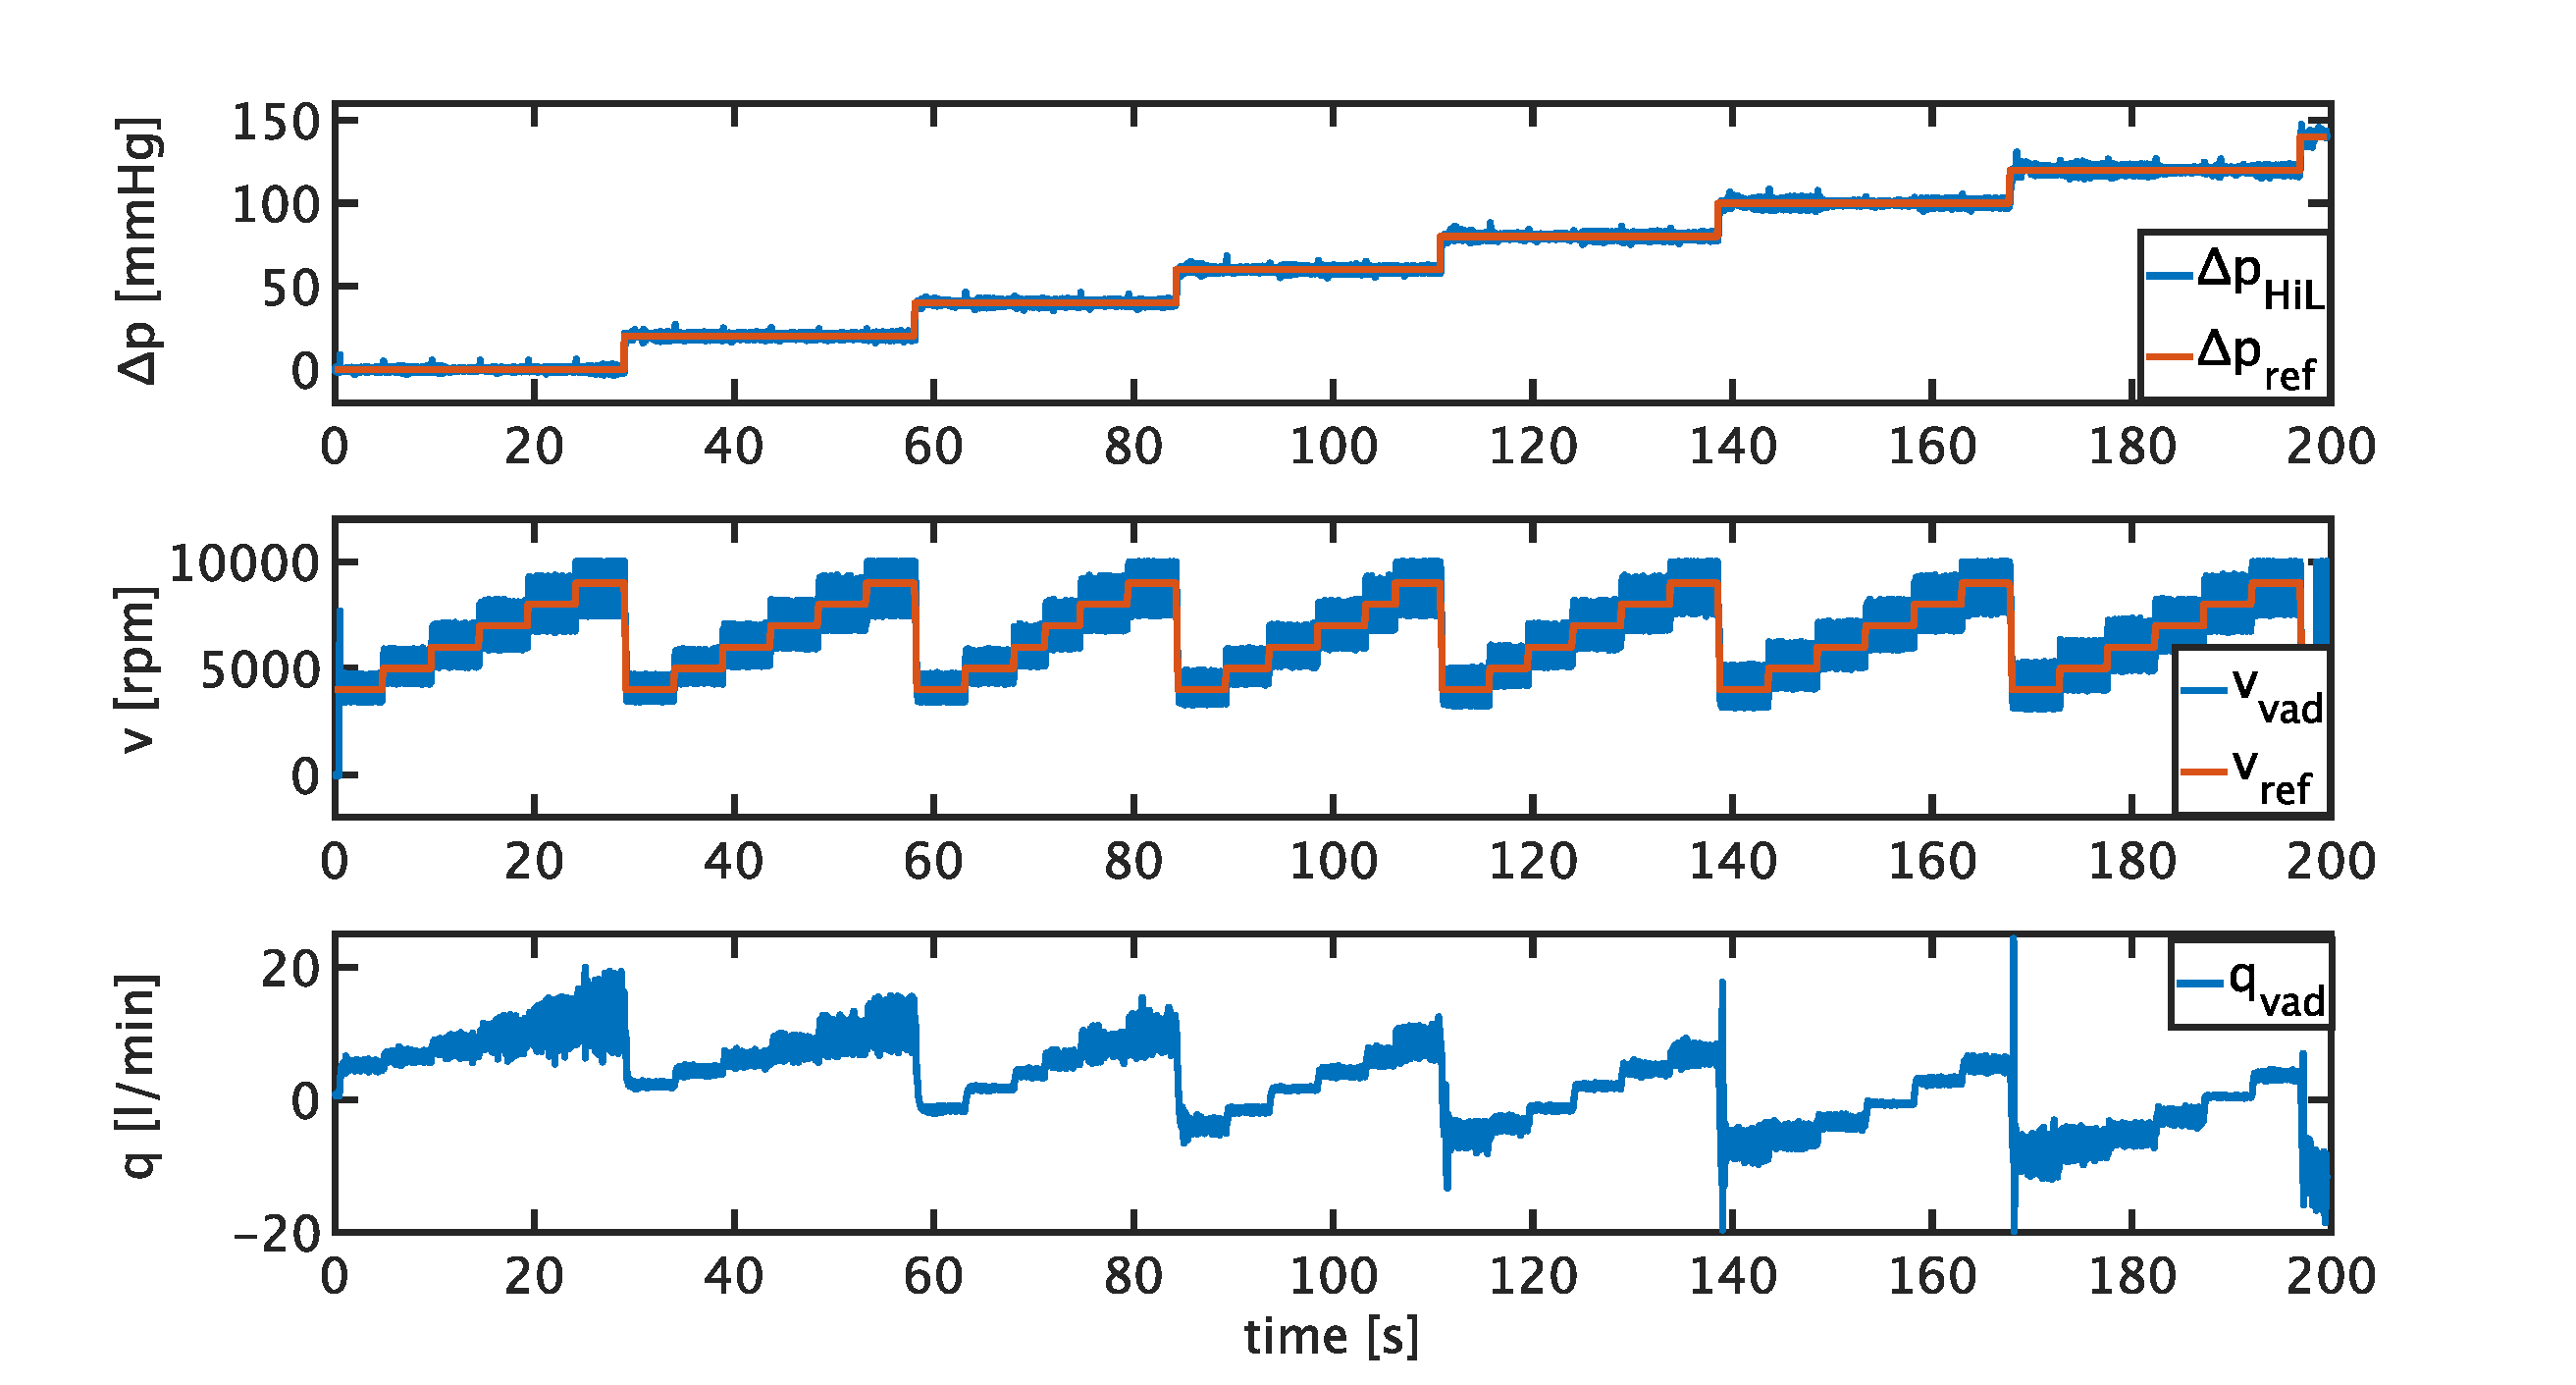
\includegraphics[width=\textwidth]{images/chapt_4/Test_60w40g_long.pdf}
  \caption[Signal curves for creation of the static map.]{Signal curves for creation of the static map for $60\,\%$ water, $40\,\%$ glycerin solution with $15 \, cm$ long tubes. Top: differential pressure, middle: rotational speed, bottom: flow through VAD.}
  \label{fig:test_60w40g_long}
\end{figure}
To determine the static map, the flow data is first broken down into individual parts corresponding to the various differential pressure levels.  These are then split into data sections for each velocity rate. Finally, the mean of the last quarter of each section is calculated. The average flow values are then displayed as a function of the differential pressure. The values of each velocity level are connected with each other.
\\At the beginning of the practical work, the Sputnik VAD was connected to the test stand via tubes of about $30\, cm$ length on both sides. Since in clinical use the pump is implemented in the patient's body and connected to the left ventricle and aorta, the tube length was not representative of a real application. To test the effect tube length has on the operating range of the pump, three different tube lengths for attachment of the VAD to the test rig are compared. The measurements have been performed with tubes of approximately $5\, cm$, $10\, cm$ and $15\, cm$ length. \figurename~\ref{fig:60w_40g} depicts the static maps for all three tube lengths measured with a fluid solution of $60\, \%$ water $40\, \%$ glycerin.
\begin{figure}[ht]
  \centering
  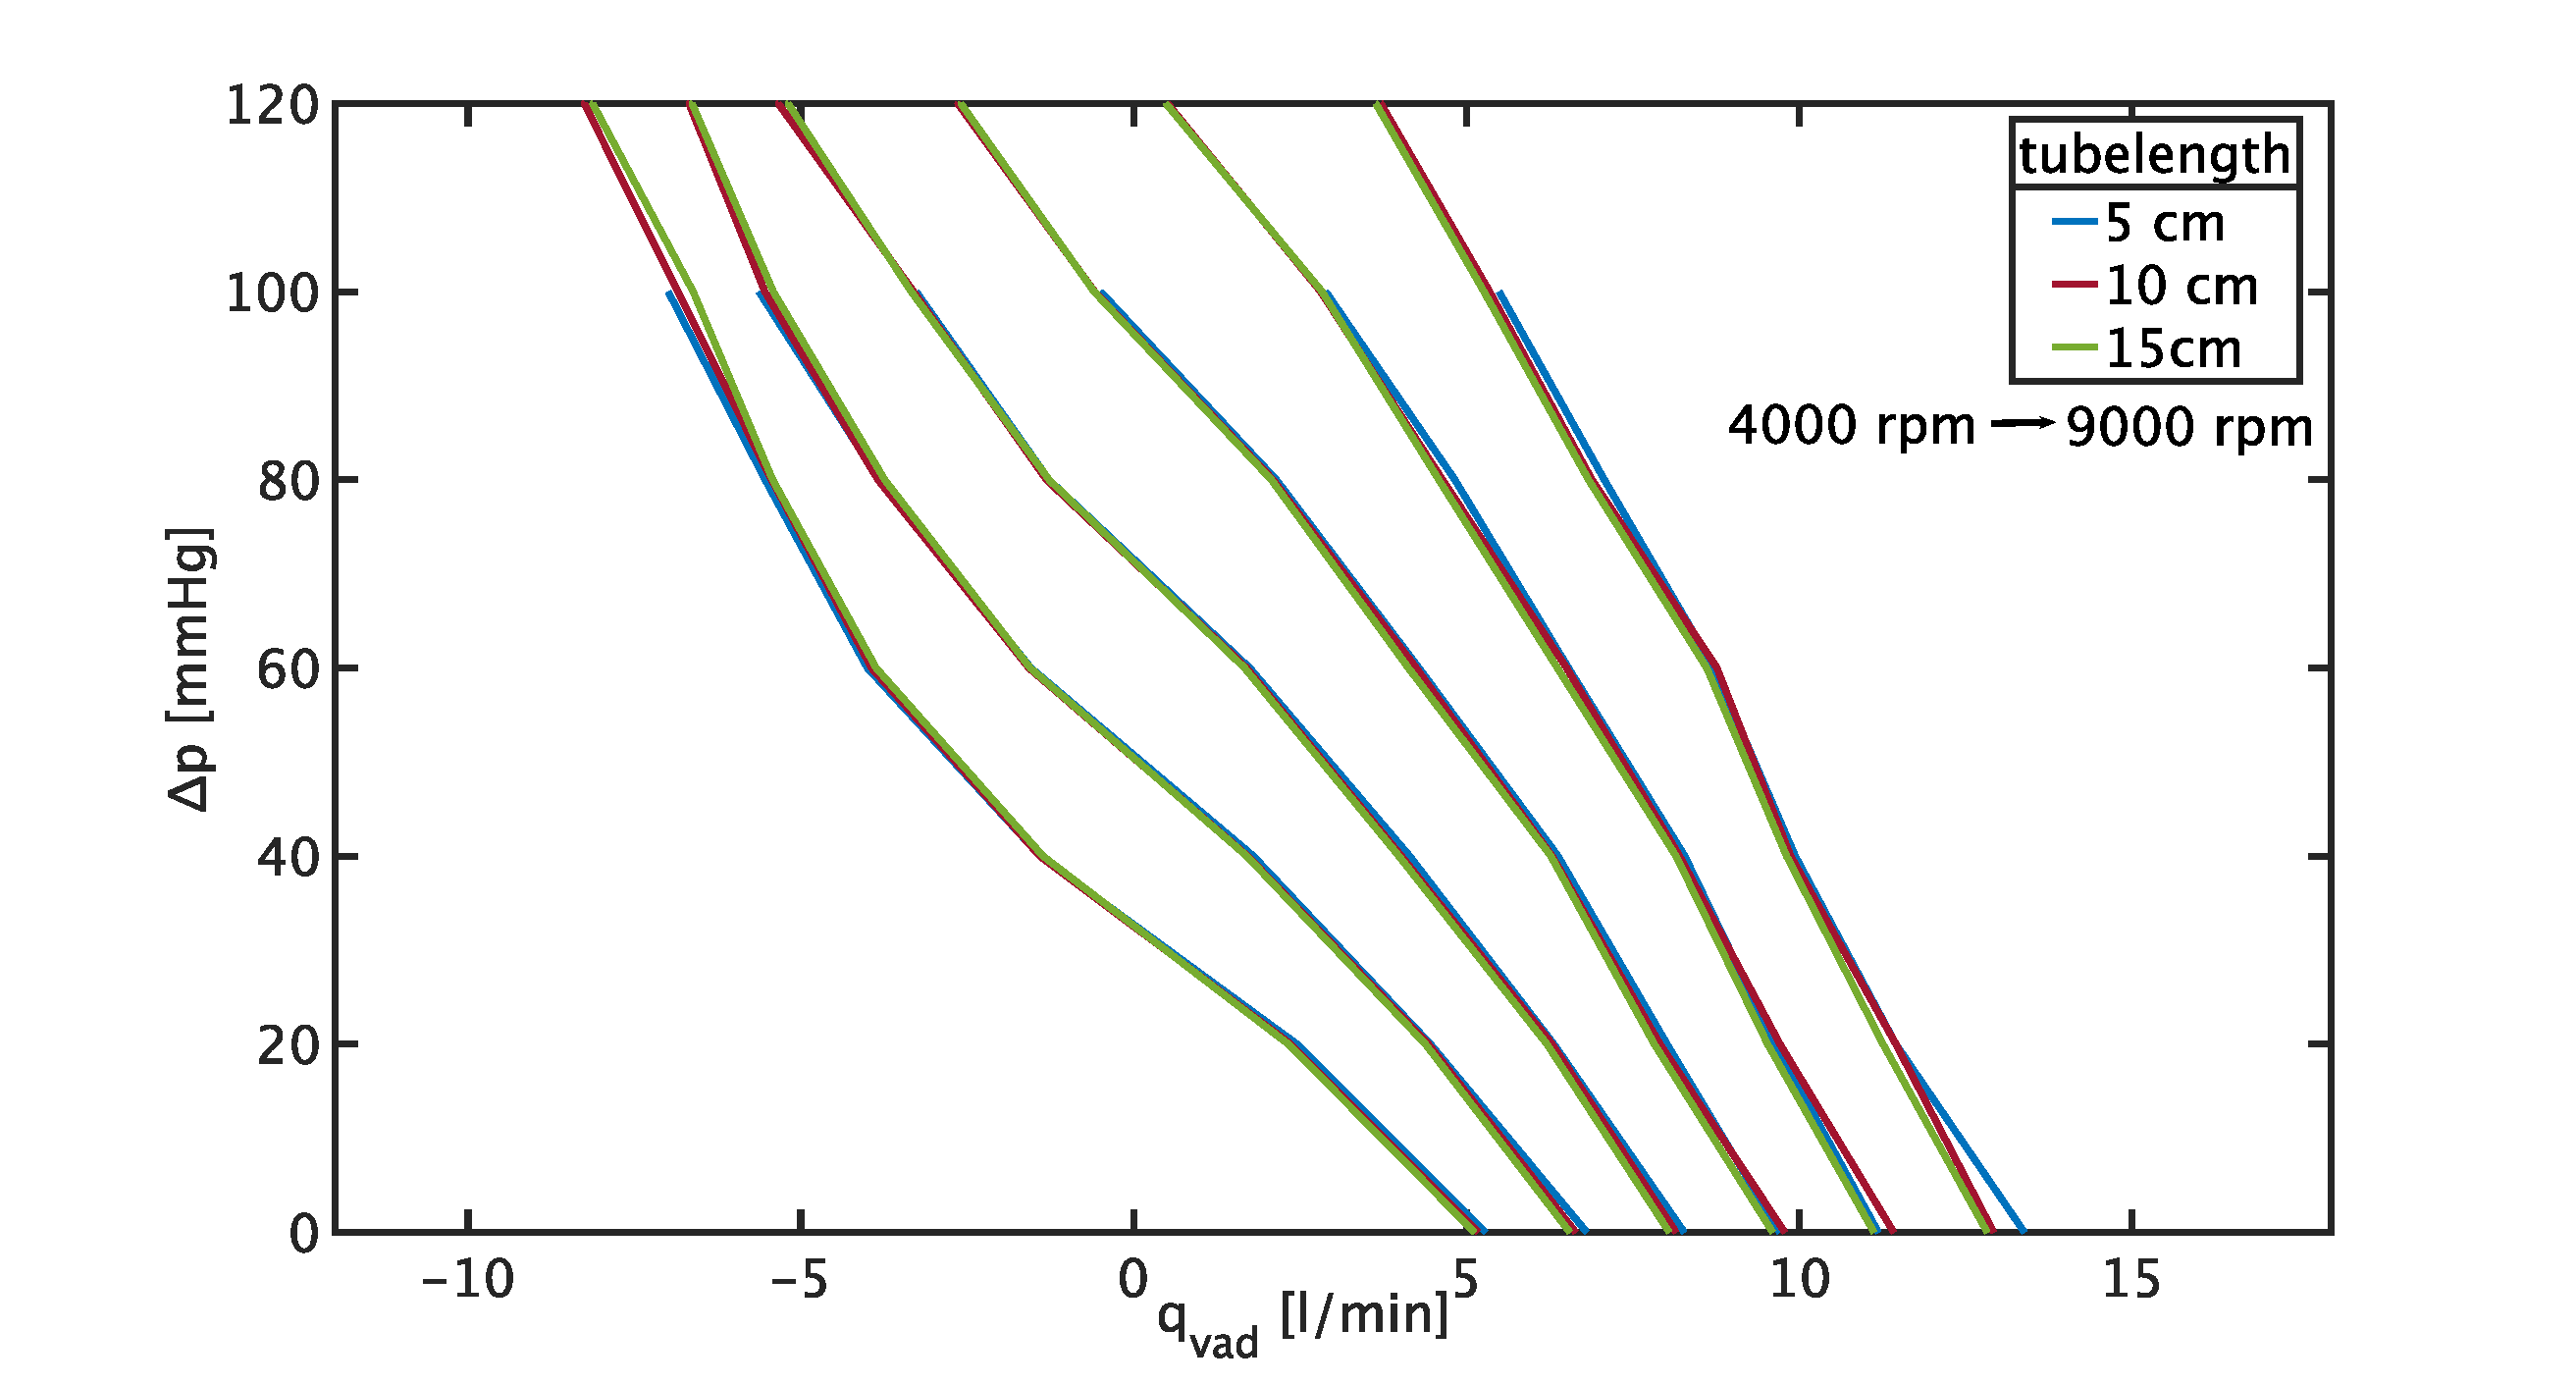
\includegraphics[width=\textwidth]{images/chapt_4/60w40g_tube_length_new.pdf}
  \caption[Static map for different tube length in 60 \% water 40 \% glycerin solution]{Static map for varying tube length in 60 \% water 40 \% glycerin solution.}
  \label{fig:60w_40g}
\end{figure}
\\Under inspection of the blue curves corresponding to a tube length of $5\, cm$ it is evident that measurements in this case were only performed up to a differential pressure of $\Delta{p}=100 \, mmHg$. This is a result of the abrupt change in differential pressure and reference speed, which lead to spontaneous reduction of the flow, up to high backflow values through the pump. Cause by this change, the pump's rotor comes to a stop. Due to higher resistance as a result of longer tubes, this event occurs only at a differential pressure of $\Delta{p}=140\, mmHg$ for the cases of $10\, cm$ and $15\, cm$ length. However, the deviation of the curves is insignificant when comparing the results for all three cases. Due to this for the implementation of flow control, the tubes of $15\, cm$ length were chosen for reasons of improved handling of the MCL. \figurename~\ref{fig:anh_1} to \figurename~\ref{fig:anh_3} in the appendix show comparisons of the static maps for varying tube length in different mixing ratios of water and glycerin.
\begin{figure}[ht]
  \centering
  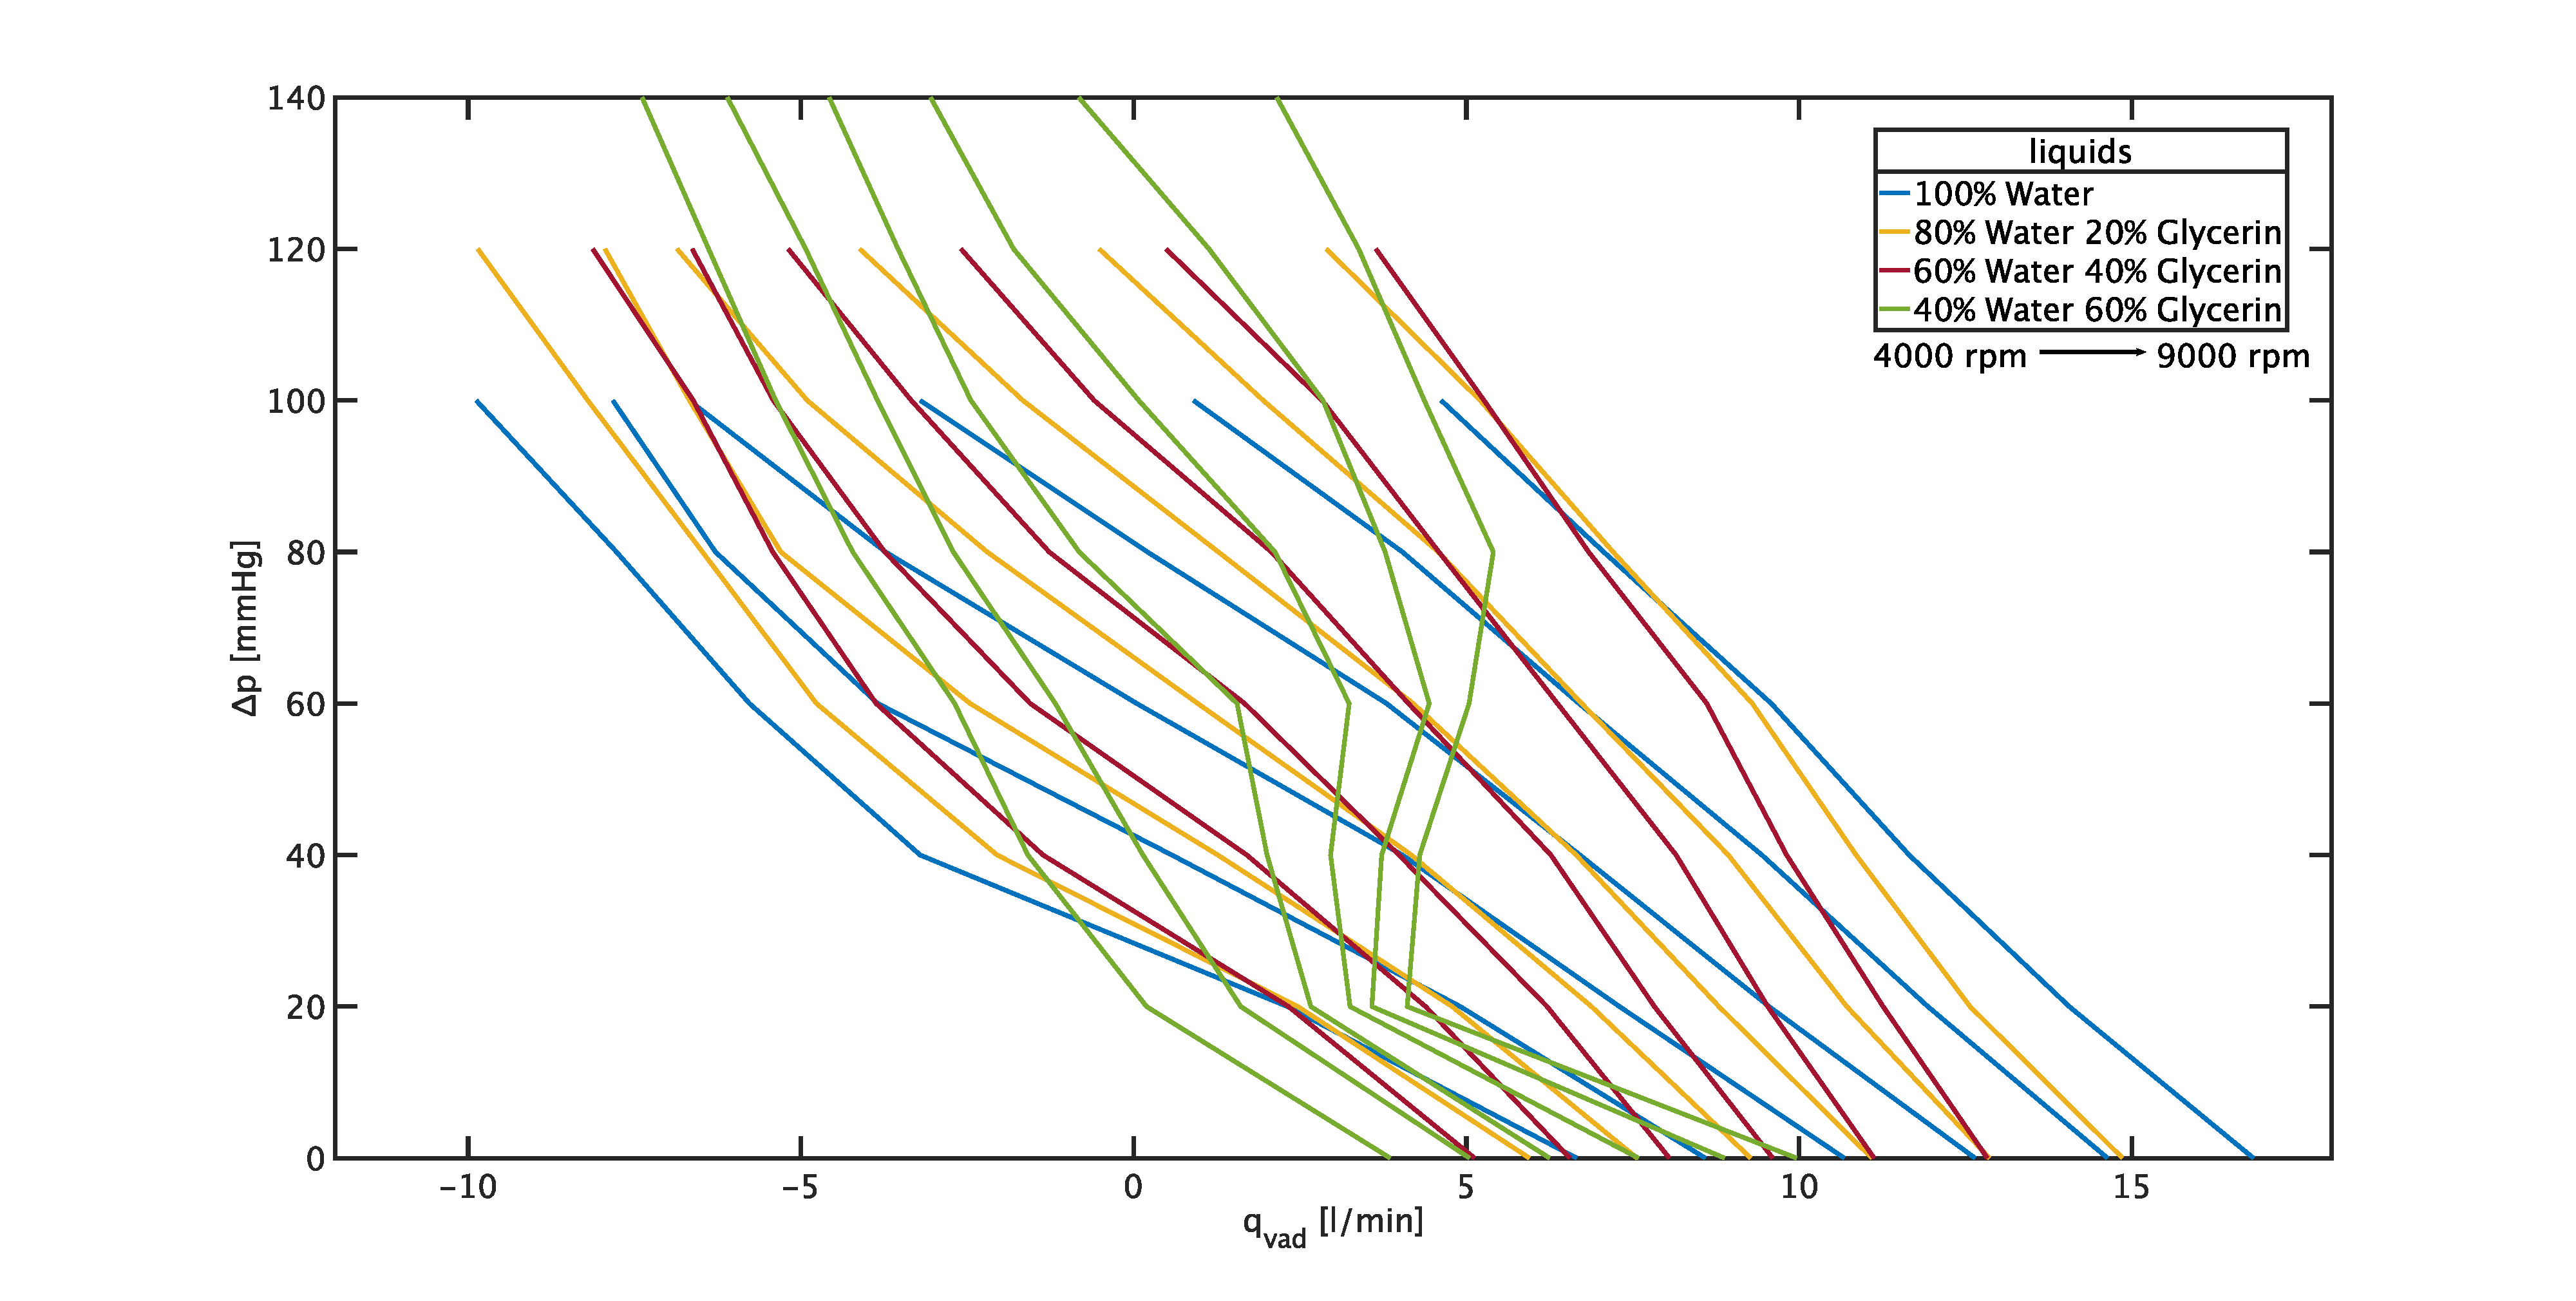
\includegraphics[width=\textwidth]{images/chapt_4/long_liquid_change_new.pdf}
  \caption[Static map for varying fluid solution with $15\,cm$ long tubes]{Static map for varying fluid solutions with $15\,cm$ long tubes.}
  \label{fig:long_tubes}
\end{figure}
\\In addition to different tube lengths, a further preliminary investigation was carried out with regard to the influence of the test liquid used. The same measurements for determination of the static map were performed in pure water, a solution of $80\, \%$ water $20\, \%$ glycerin, a solution of $60\, \%$ water $40\, \%$ glycerin and a solution of $40\, \%$ water $60\, \%$ glycerin. Representing the static maps for all four solutions measured with tubes of $15\, cm$ length, \figurename~\ref{fig:long_tubes} discloses significant deviations between the fluids. Since the resistance of the liquid falls with decreasing proportion of glycerin in the solution, differences in reachable differential pressure occure due to the aforementioned reason of spontaneous flow reduction. However, as the fluid resistance increases, the pumpable flow also decreases. All further measurements of this thesis are performed for a solution of $60\, \%$ water $40\,$ glycerin as this mixture most closely reflects the properties of blood.
\figurename~\ref{fig:anh_4} and \figurename~\ref{fig:anh_5} in the appendix depict comparisons of the static maps for varying  solutions with $5\, cm$ and $10\, cm$ tube length.
The resulting static map for the chosen final setup of the MCL is depicted in \figurename~\ref{fig:60w40glong}.

\begin{figure}[ht]
  \centering
  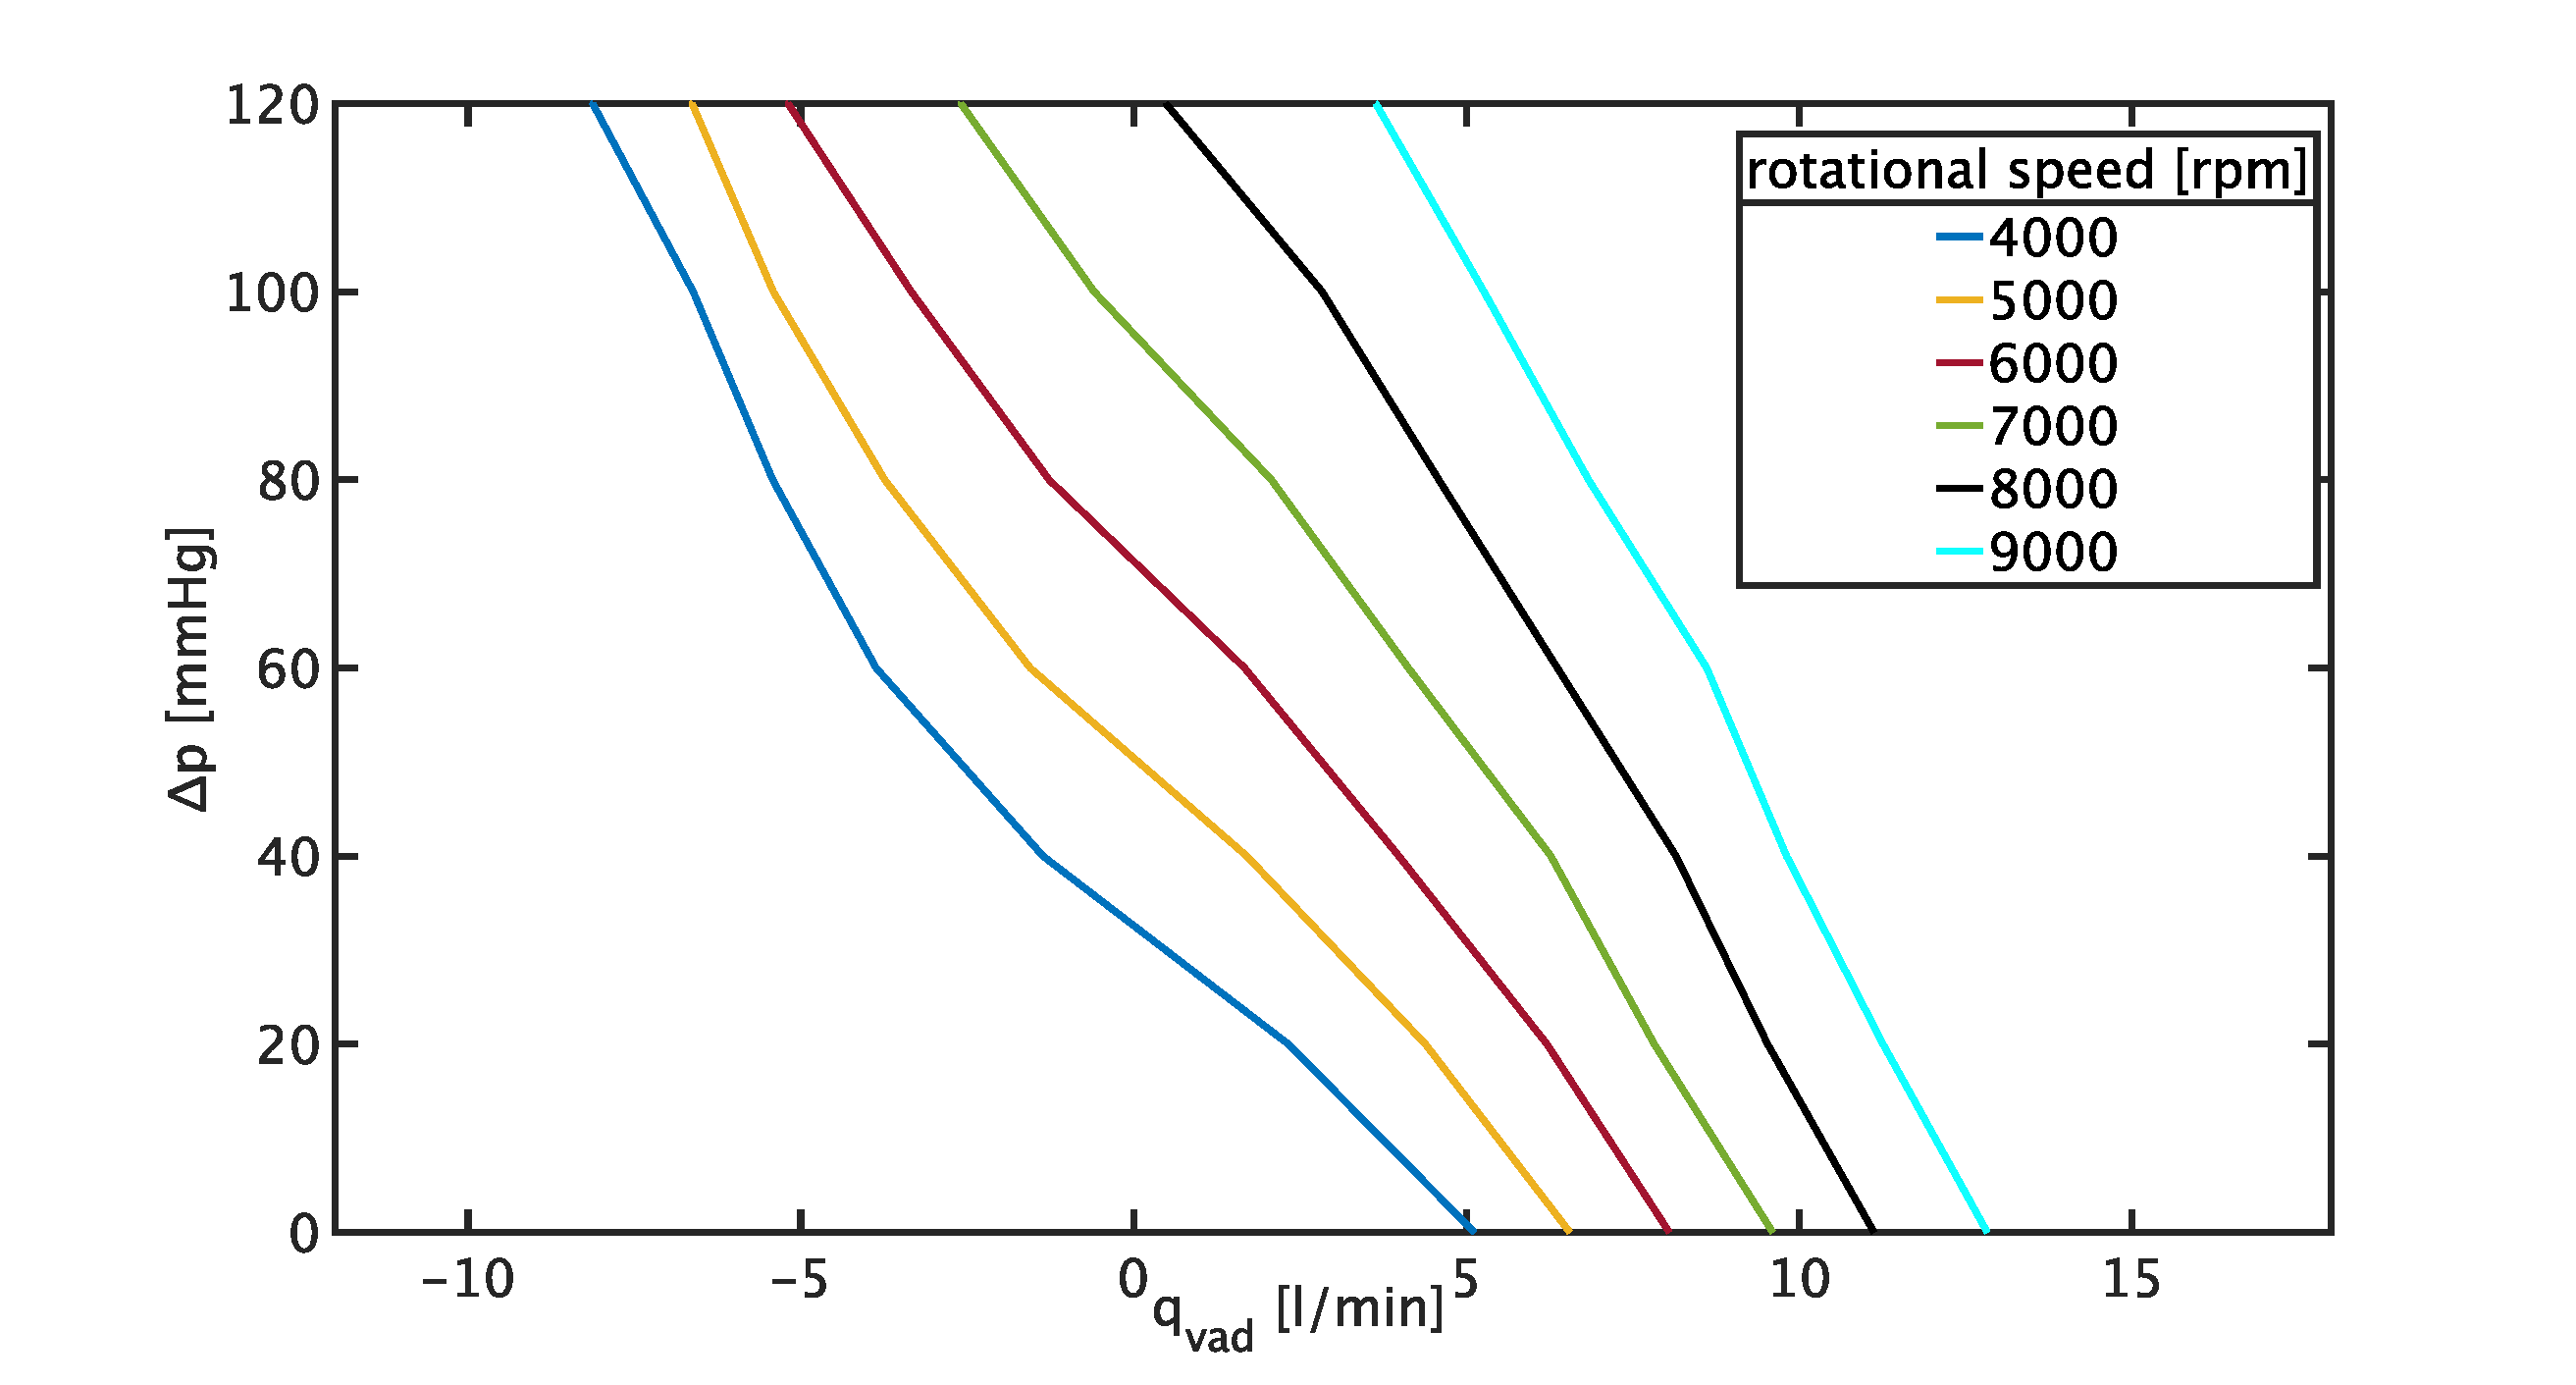
\includegraphics[width=\textwidth]{images/chapt_4/60w40g_long.pdf}
  \caption[Static map for solution of $60\, \%$ water $40\, \%$ glycerin with $15\,cm$ long tubes]{Static map for solution of $60\, \%$ water $40\, \%$ glycerin with $15\,cm$ long tubes.}
  \label{fig:60w40glong}
\end{figure}

%% close up von einem 1k Sprung zur Auslegung der Plant im durch 4.7 definitierten positiven Fluss Bereich.
%% Vergleich des gemessenen Signals mit simuliertem Signal.
As part of the system identification, the transfer function of the Sputnik VAD is determined. For this purpose, the step response of the pump to a $1000\,rpm$ step in reference speed is analyzed.
\\Initially, the measured flow values from the static map determination measurement are prepossessed by using a $2^{nd}$-order butterworth filter with a cut-off frequency of $f_c = 5\,Hz$ and sampling frequency $f_s=1000 \, Hz$. For determination of the transfer function, filtered flow for an increase from $v_{ref,low}=5000\,rpm$ to $v_{ref,high}=6000\,rpm$ in reference speed at a differential pressure of $\Delta{p}=40\,mmHg$ is analyzed. The blue line in \figurename~\ref{fig:plant} depicts the filtered flow for this measurement. It is evident, that the system's behavior can be approximated by a $PT_1$-element.
 The characteristic parameters of the transfer function according to equation (\ref{eq:tf_pt1}) are represented in \figurename~\ref{fig:plant}. The static gain $k_s$ is determined as
\begin{equation}
%  \begin{split}
  k_s = \frac{k_{high}-k_{low}}{v_{ref,high}-v_{ref,low}}=0.0018
  %\\ = \frac{2.3008 - 0.4672}{6000 - 5000} = 0.0018.
%  \end{split}
\label{eq:k_s_1}
\end{equation}
with $k_{high}=2.3008$ and $k_{low}=0.4672$. The time constant T is determined to $T=0.081$.
According to equation (\ref{eq:tf_pt1}) the transfer function for the plant results in
\begin{equation}
    G(s) = \frac{0.0018}{1+0.081s}.
 \label{eq:plant}
\end{equation}
\begin{figure}[ht]
  \centering
  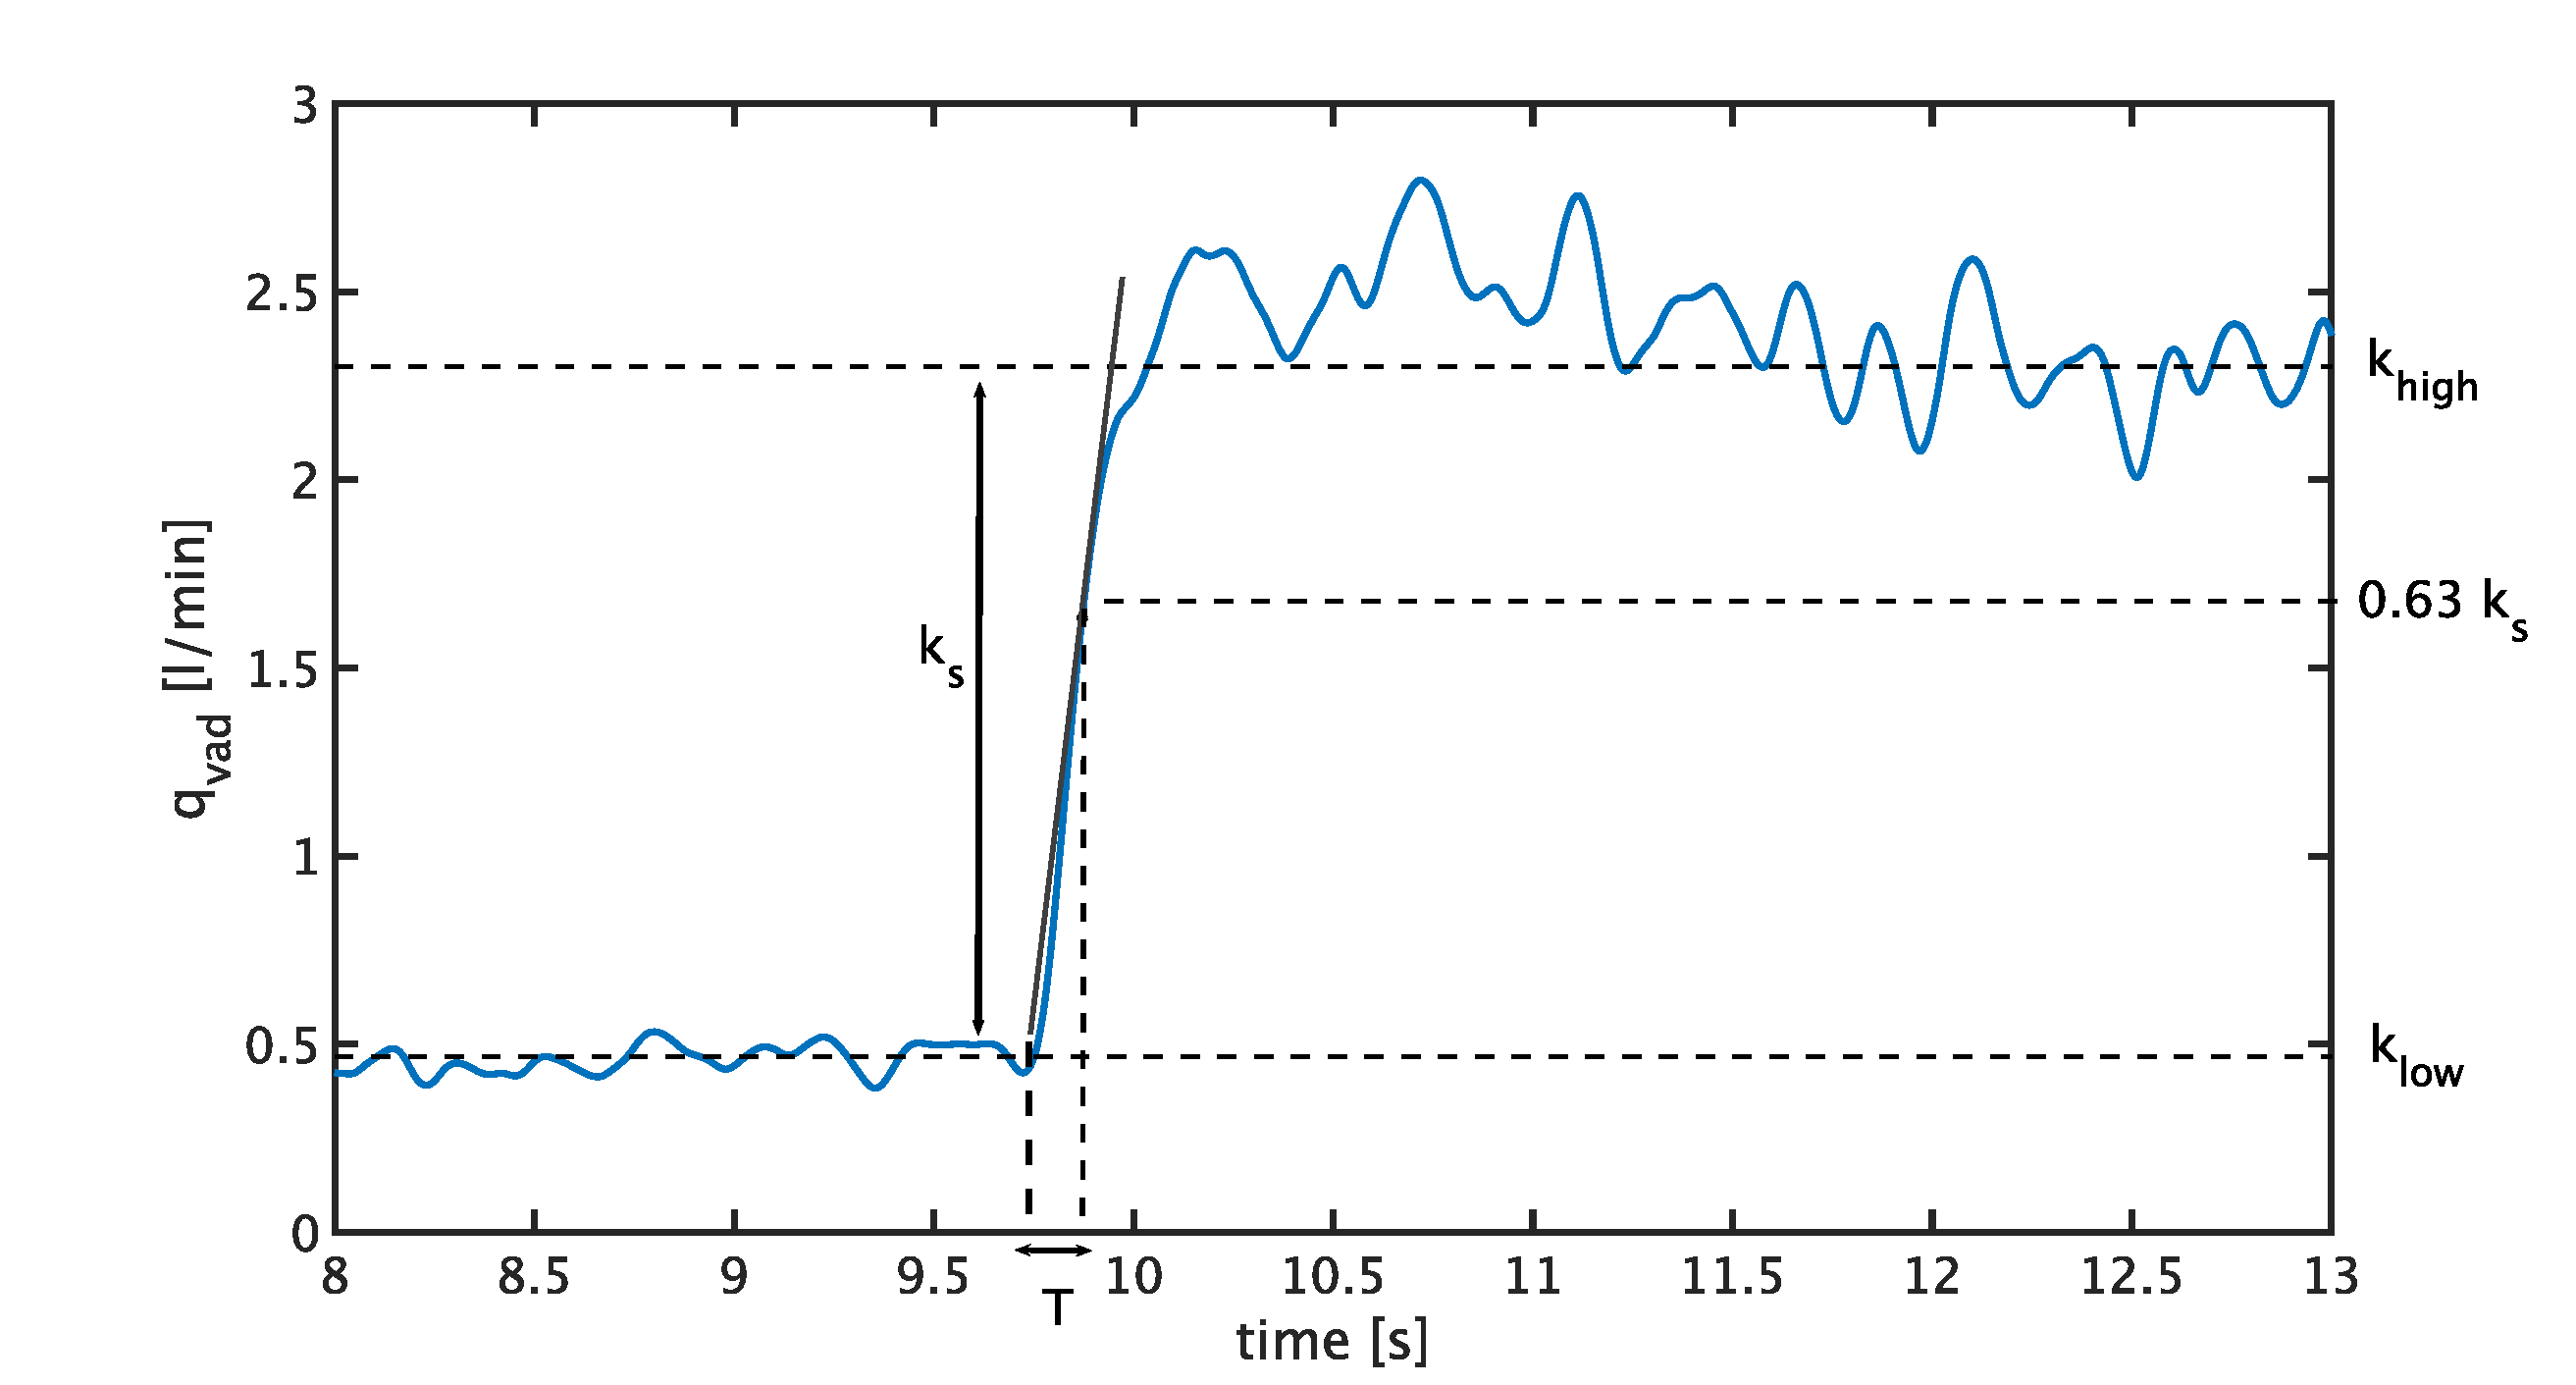
\includegraphics[width=\textwidth]{images/chapt_4/plant_generation.pdf}
  \caption[Transfer function of Sputnik VAD]{Step in flow, triggered by a step in reference speed by 1000 rpm with identification of the variables for determining the transfer function of a $PT_1$ element.}
  \label{fig:plant}
\end{figure}
